\subsection{Printed Circuit Board}
A PCB is a required part of our design. Therefore, it will be critical to understand the details of how PCB functions so that we can best translate our circuit design on to one. There are many different parameters that go into PCB that we discuss in the following section.

\subsubsection{What is a PCB?}
Before we get into the details of the PCB design first lets go over what exactly is a PCB or a printed circuit board. When computers were first constructed they took up massive rooms and could provide much less processing power than they could today. However after decades on innovation and inventions we can now fit more processing power than the original space shuttles comfortably in our pockets. One such invention is the PCB. In appearance a PCB resembles a flat green board but under a microscope there is so much more detail. Within a PCB there are several layers that make up its form and function. The first one is the mounting components. These are the top most and bottom most layers that provide placement for various components such as microchips, resistors, capacitors or anything else that may require placement on the PCB. The next two layers well discuss are the power plane and ground plane. As their name suggests these provide power and ground respectfully to any components that require as such. Finally we have the signal trace layers. These layers are composed of copper, insulating fiberglass, and an epoxy resin that prevents any flow of electricity. PCB usually are composed of anywhere in between 2-50 signal trace layers as these layers connect components of the PCB to one another. 

Now that we know that PCBs are comprised of layers that provide power, ground, and communication between devices on the motherboard an appropriate question to ask is how layers connect to one another between the insulating material. This is due to VIA's or Vertical Interconnect Access. VIAs are drilled and metal plated holes that are used to connect two or more layers on the PCB. There are three types of VIAs those being a through hole, blind VIA, and buried VIA. A through hole goes completely through the PCB from the top layer to the bottom layer. A blind VIA connects the top or bottom layer to a layer part way through the PCB. Finally buried VIAs connect two or more central layers. 

\subsubsection{PCB Function}
PCBs are integral to almost every modern day electrical system. A PCB allows seamless and streamlined communication between system components, effortless powering of circuits, and allows for a much more compact design for any electrical system need. Utilizing a PCB's revolutionary design no longer must we struggle with large and confusing circuit designs. Using trace layers the phone in your pocket uses enough copper wire to span the distance of an entire football field. Not only that but trace layers can be compacted to stack on top of one another allowing electrical connections to pass by one another in very direct manors. All in all while a PCB is not necessary to make circuit designs work, without them any system that could otherwise be implemented on a PCB would be many more times the size and complex to construct.

\subsubsection{Our PCB Design}
When selecting the parameters of our PCB some information must decided upon. Selections we must decide on are RF routing, number of layers, trace thickness, and SMD passive sizes. The first decision well make is on trace thickness because of how straight forward it is. A good rule of thumb is 1 mil(one thousandth of an inch) is usually required for 1 amp, as a result because the maximum current we can expect is 3 amps we should have our trace thickness be 3 mil. Due to the number of components with a high number of pins and just overall number of items well be trying to fit in a compact state its been decided having a pin density of around 0.5 would be best. As a result well be utilizing a 4 signal layer PCB. When it comes to SMD passive sizes the SMDs well be looking at can come in many package types which will make the SMDs anywhere from 0.4x0.2(mm) to 7.4x5.1(mm). However for this project it has been decided that with our project needs the desirable package type creates an SMD with a size of 2.0x1.3(mm)(SMD package type 0805). This will allow us to keep the design compact while also make construction more streamlined as any smaller would create more difficulties. Additionally this package type specializes in resistors and capacitors which makes up a majority of our circuit design.

Finally we must decided on RF routing. The beginners essential to RF design is minimizing cross talk. This is when more than one RF signal can tamper with one another due to E and H fields. The way well minimize this is by utilizing our 4 trace layer design. While the two inner most trace layers will be dedicated to low speed digital signals the top and bottom trace layers will be dedicated to our RF planes. This will provide an adequate amount of space between layers that will eliminate cross talk allowing the board to effectively separate the signals. With all this together we can put a picture together of what our PCB should resemble. Figure \ref{fig:PCB} is a prototype PCB layout that will eventually evolve into a fully functional design that will enable our device to operate compactly, efficiently, and seamlessly.

\begin{figure}
    \centering
    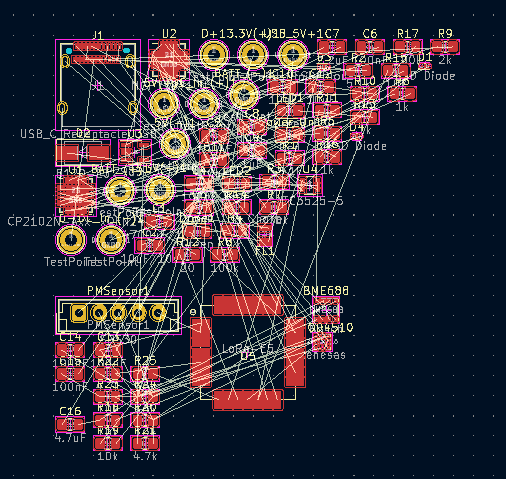
\includegraphics[width=4.3in]{figures/PCB.png}
    \caption{Our initial PCB design}
    \label{fig:PCB} 
\end{figure}


